\documentclass[12pt]{article}

%% Packages

% obligatory math environments, symbols, and theorems
\usepackage{amsmath, amssymb, amsthm}

% sometimes you gotta draw stuff, like _c_ommutative _d_iagrams.
\usepackage{tikz, tikz-cd}

% sometimes you gotta write code
\usepackage{listings}


%% Environments

\newtheorem{thm}{Theorem}

\theoremstyle{definition}
\newtheorem{defn}{Definition}


%% Aliases
\newcommand{\N}{\mathbb{N}}
\newcommand{\Z}{\mathbb{Z}}
\newcommand{\Q}{\mathbb{Q}}
\newcommand{\R}{\mathbb{R}}

\newcommand{\del}{\partial}

\newcommand{\mono}{\hookrightarrow}
\newcommand{\epi}{\twoheadrightarrow}

\newcommand{\dirlim}{\varinjlim}
\renewcommand{\projlim}{\varprojlim}

\begin{document}
  \section{Intro}

  This entire project came about from trying to generalize the standard
  algorithm for addition in $\Z$. We work one column at a time, and 
  addition in one column takes place in a finite group ($\Z / 10$).
  However, we occasionaly have to ``carry'' the output from one column's
  computation into the next column, so addition in previous columns can
  impact the addition of future columns.

  The \emph{automatic} interpretation is that addition in $\Z$ can be 
  computed using a \textbf{Finite State Automaton} (shown below). This is
  a fairly powerful requirement, as it says that addition in $\Z$ is 
  essentially as easy as addition in $\Z / 10$. We only have to remember
  one piece of information at a time (namely what we are carrying).

  \begin{center}
    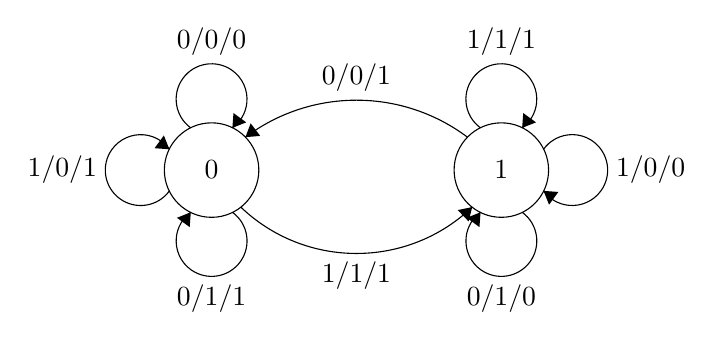
\begin{tikzpicture}[scale=0.2]
    \tikzstyle{every node}+=[inner sep=0pt]
    \draw [black] (17.3,-28.3) circle (3);
    \draw (17.3,-28.3) node {$0$};
    \draw [black] (35.7,-28.3) circle (3);
    \draw (35.7,-28.3) node {$1$};
    \draw [black] (33.85,-30.649) arc (-46.30625:-133.69375:10.639);
    \fill [black] (33.85,-30.65) -- (32.93,-30.84) -- (33.62,-31.56);
    \draw (26.5,-34.1) node [below] {$1/1/1$};
    \draw [black] (38.38,-26.977) arc (144:-144:2.25);
    \draw (42.95,-28.3) node [right] {$1/0/0$};
    \fill [black] (38.38,-29.62) -- (38.73,-30.5) -- (39.32,-29.69);
    \draw [black] (14.62,-29.623) arc (324:36:2.25);
    \draw (10.05,-28.3) node [left] {$1/0/1$};
    \fill [black] (14.62,-26.98) -- (14.27,-26.1) -- (13.68,-26.91);
    \draw [black] (15.977,-25.62) arc (234:-54:2.25);
    \draw (17.3,-21.05) node [above] {$0/0/0$};
    \fill [black] (18.62,-25.62) -- (19.5,-25.27) -- (18.69,-24.68);
    \draw [black] (18.623,-30.98) arc (54:-234:2.25);
    \draw (17.3,-35.55) node [below] {$0/1/1$};
    \fill [black] (15.98,-30.98) -- (15.1,-31.33) -- (15.91,-31.92);
    \draw [black] (19.445,-26.214) arc (126.88367:53.11633:11.754);
    \fill [black] (19.45,-26.21) -- (20.39,-26.13) -- (19.78,-25.33);
    \draw (26.5,-23.36) node [above] {$0/0/1$};
    \draw [black] (37.023,-30.98) arc (54:-234:2.25);
    \draw (35.7,-35.55) node [below] {$0/1/0$};
    \fill [black] (34.38,-30.98) -- (33.5,-31.33) -- (34.31,-31.92);
    \draw [black] (34.377,-25.62) arc (234:-54:2.25);
    \draw (35.7,-21.05) node [above] {$1/1/1$};
    \fill [black] (37.02,-25.62) -- (37.9,-25.27) -- (37.09,-24.68);
    \end{tikzpicture}
  \end{center}
  Here an edge from $p$ to $q$ labelled $a / b / c$ to mean that, 
  given inputs $a$ and $b$, while in state $p$, we should output $c$
  and transition to $q$. Intuitively, the states correspond to what we 
  are currently carrying.  It is clear that this machine does actually
  compute the basic addition algorithm in base 2, provided one starts in state 
  $0$. While an analogous machine exists for the computation in base 10, it is 
  somewhat more cumbersome to draw.

  The \emph{cohomological} interpretation is that addition in $\Z$ can be
  approximated by addition in $\Z / 10^n$, provided we are adding integers
  of length at most $n-1$. When adding integers of length $n$, 
  $\Z / 10^n$ does not (in general) correctly compute the sum in $\Z$,
  since the sum of two $n$ digit numbers may result in a sum of length $n+1$,
  which $\Z / 10^n$ cannot represent. This ``error'' is captured by a function
  $\rho_n : \Z / 10^n \times \Z / 10^n \to \Z / 10$, which returns the 
  overflow digit. These $\rho_n$ satisfy the \emph{Cocycle Condition}, and
  witness $\Z / 10^{n+1}$ as a $\Z / 10$-by-$\Z / 10^{n+1}$ group extension.

  This says that every element of $\Z / 10^{n+1}$ can be written as 
  $(d,ds)$ where $d \in \Z / 10$ and $ds \in \Z / 10^n$. 
  Then we can compute the $\Z / 10^{n+1}$ addition $(x,xs) + (y,ys)$ by 
  inductively computing $xs + ys \in \Z / 10^n$ and then computing 
  $x + y + \rho_n(xs,ys) \in \Z / 10$.

  This perspective then lets us write addition in $\Z$ as the limit of 
  addition in each of these approximations. Formally $\Z$ is the 
  ``finite-support subgroup'' in the projective limit $\projlim \Z / 10^n$.

  \bigskip

  With this perspective in mind, it is natural to ask if we can draw this 
  parallel in other settings. That is, for some finite abelian group $G$
  equipped with a cocycle $\rho : G \times G \to G$ 
  (denoting a generalized ``carry'' function), can we construct a new group by 
  iteratively adding and carrying ``one column at a time'' analogous to
  realizing $\Z$ (actually the $10$-adics\ldots) as a projective limit of 
  fixed-length approximations? If so, one would expect this limit group to
  admit an automatic structure which computes its addition in a finitary way,
  analogous to the standard addition algorithm for $\Z$.

  We give positive answers to both of these questions, and constructive 
  proofs of the relevant automata.

  \section{Cohomology}
  Let $G$ be a finite abelian group, and $\rho : G \times G \to G$ a 
  2-cocycle satisfying a coherence condition ($\star$), which we define below. 
  We will inductively define $G_n$ by iterating group extensions,
  where each $\rho_n : G_n \times G_n \to G$ is ``essentially the same'' as
  the provided $\rho$. The structure of these group extensions will provide the
  data required for a projective limit, which will end up being an automatic
  structure. 
  
  Somewhat surprisingly, we can \emph{also} find cocycles 
  $\rho_n' : G \times G \to G_n$, which are also ``essentially the same'' as
  the provided $\rho$. However, these induce the data of a direct limit,
  which is infinite torsion, but still automatic 
  (indeed the same automaton will compute addition in the direct and 
  proejctive limits). This is analogous to using essentially the same addition
  algorithm to compute in $\dirlim \Z / 10^n$, the subgroup of $S^1$ given by
  rationals with denominator a power of $10$.

  Perhaps \emph{even more} surprisingly, proving the projective limit case
  directly seems to be extremely difficult, and so we pass through the 
  injective construction as part of the proof. Some intuition for why this
  is the case will be provided before the proof of the existence of the 
  projective limit, though we will start with the injective case as it is simpler.

  \subsection{Injective Limit}

  Let $G$ be an abelian group, and $\rho : G \times G \to G$ a 2-cocycle.
  We demand $\rho$ additionally satisfy the coherence condition below:

  \[ 
    \forall a,b,c \in G. 
    \rho \left ( \rho(a,b), \rho(a+b,c) \right )
    = 
    \rho \left ( \rho(b,c), \rho(a,b+c) \right ) 
    \tag{$\star$}
  \]

  Note: All of our group extensions will come with trivial action.
  For a group extension $K \mono G \epi Q$ with cocycle 
  $\rho : Q \times Q \to K$, we identify $G$ with $Q \times K$
  and addition $(q_1,k_1) + (q_2,k_2) = (q_1 + q_2, k_1 + k_2 + \rho(q_1,q_2))$.

  \begin{thm}
    We can inductively define group extensions $G_n \mono G_{n+1} \epi G$
    with cocycles $\rho_n' : G \times G \to G_n$ ``essentially the same'' as 
    $\rho$.
  \end{thm}

  \begin{proof}
    Inductively assume we have defined $G_n$ satisfying $G_{n-1} \mono G_n \epi G$. 
    
    Define $\rho_n' : G \times G \to G_n$ by 
    $(g_1,g_2) \mapsto (\rho(g_1,g_2), 0^{n-1})$.

    To show $\rho_n'$ is a cocycle, we need to check
    $\rho_n'(a,b) + \rho_n'(a+b,c) = \rho_n'(b,c) + \rho_n'(a+b,c)$:

    \begin{align*}
    \centering
      \rho_n'(a,b) + \rho_n'(a+b,c) &= \\ 
      \rho_n'(b,c) + \rho_n'(a,b+c) \\
      &\iff \\ 
      (\rho(a,b),0^{n-1}) + (\rho(a+b,c),0^{n-1}) &= \\
      (\rho(b,c), 0^{n-1}) + (\rho(a,b+c),0^{n-1}) \\ 
      &\iff \\
      \Big ( \rho(a,b) + \rho(a+b,c),~\rho_{n-1}'(\rho(a,b), \rho(a+b,c)) \Big ) &= \\ 
      \Big ( \rho(b,c) + \rho(a,b+c),~\rho_{n-1}'(\rho(b,c), \rho(a,b+c)) \Big )\\
      &\iff \\
      \bigg ( 
        \rho(a,b) + \rho(a+b,c), 
        \Big ( \rho(\rho(a,b),\rho(a+b,c)), 0^{n-2} \Big )
      \bigg ) &= \\
      \bigg ( 
        \rho(b,c) + \rho(a,b+c), 
        \Big ( \rho(\rho(b,c), \rho(a,b+c)),0^{n-2} \Big )
      \bigg )
    \end{align*}

    The first equality is definitional. 
    The second follows from addition in $G_n$,
    and the third from the (inductive) definition of $\rho_{n-1}'$.

    Finally, at the end of it all, the two terms are indeed equal. Equality
    in the first component is the cocycle condition for $\rho$, and equality
    in the second component is exactly ($\star$).
  \end{proof}

  So now we see each $G_n \mono G_{n+1}$. Then we have a diagram:

  \begin{center}
  \begin{tikzcd}
    G_1 \mono G_2 \mono G_3 \mono G_4 \mono G_5 \mono \cdots
  \end{tikzcd}
  \end{center}

  which admits a direct limit $\overrightarrow{G}$.

  Note: While we (for the purposes of this informal discussion) leave 
  ``essentially the same'' undefined, it should be clear what is meant:
  Each $\rho_n' : G \times G \to G_n$ is just $s_n \circ \rho$, 
  where $s_n$ is the canonical (set theoretic) section $G \to G_n$ 
  since $G_n$ is also an extension of $G$.

  \subsection{Projective Limit}

  Now, to define a projective limit, we want a family of extensions
  $G \mono G_{n+1} \epi G_n$, but this requires a family of cocylces
  $\rho_n : G_n \times G_n \to G$, which represent the ``overflow'' of
  doing addition with elements with $n$-many digits. Of course, without
  knowledge of the limit (which we have in $\Z$), it is unclear how to 
  properly define $\rho_n$\ldots Intuition and formal manipulations suggest

  \[
    \rho_{n+1}((x,a),(y,b)) = \rho(a,b) + \rho(a+b, \rho_n(x,y))
    \tag{1}
  \]
  is the right definition (Here $x,y \in G_n$ and $a,b \in G$). 

  Somewhat unfortunately, a direct proof that these $\rho_n$ are all cocycles
  seems difficult. Thankfully, intuition \emph{also} suggests that the $G_n$
  should be the same as in the injective case, and it is only the limiting
  behavior that differs. We will prove this intuition correct, and then use
  it to cheat and indirectly prove the $\rho_n$ are cocylces.

  \begin{thm}
    If $G_n \mono G_{n+1} \epi G$ is a group extension as in the previous
    section, then $G \mono G_{n+1} \epi G_n$ is \emph{also} a group extension.
  \end{thm}

  \begin{proof}
    Say $G_n \mono G_{n+1} \epi G$ is an extension as above, and 
    inductively assume we can write $G_n$ as an extension
    $G \mono G_n \epi G_{n-1}$.

    Consider $\varphi : G_{n+1} \epi G_n$ by 
    $(g_1, g_2, \ldots, g_n, g_{n+1}) \mapsto (g_1, g_2, \ldots, g_n)$.

    It is shockingly non-routine to verify $\varphi$ is indeed a group hom, 
    so a proof is included here:

    Say $\alpha, a, \beta, b \in G$ and $x,y \in G_{n-1}$:

    \begin{align*}
      \varphi((\alpha, xa) + (\beta, yb)) 
      &= \varphi((\alpha + \beta, xa + yb + \rho_n'(\alpha,\beta))) 
        && \text{addition in $G_{n+1}$}\\
      &= \varphi((\alpha + \beta, (x + y + \rho(\alpha,\beta)0^{n-1}, a + b + \text{stuff})))
        && \text{inductive addition in $G_n$}\\
      &= (\alpha + \beta, x+y+\rho(\alpha,\beta)0^{n-1})
        && \text{defn $\varphi$}\\
      &= (\alpha, x) + (\beta, y)
        && \text{addition in $G_n$}\\
      &= \varphi((\alpha,xa)) + \varphi((\beta,xb))
    \end{align*}

    Importantly, the addition on lines 2 and 4 both take place in $G_n$, 
    though we are switching our representation. On line 2, we consider
    $G_n$ inductively as $G \mono G_n \epi G_{n-1}$, while in line 4 we
    consider $G_n$ as in the previous section, $G_{n-1} \mono G_n \epi G$.
    Also, importantly, the ``stuff'' in line 2 comes from whatever
    magic $\rho_{n-1} : G_{n-1} \times G_{n-1} \to G$ happens to do. While
    we do \emph{technically} give a constructive definition of the $\rho_n$,
    actually figuring out what they do is a real pain. Thankfully, $\varphi$
    immediately kills whatever stuff we happen to collect!

    Back to the proof at hand, it is clear that the kernel of $\varphi$ is
    $\{0^ng~|~g \in G \}$, which is clearly isomorphic to $G$ as a group. 
    Thus $G \mono G_{n+1} \epi G_n$ is an extension! 
  \end{proof}

  Dual to before, these group extensions give rise to a diagram:

  \begin{center}
  \begin{tikzcd}
    \cdots \epi G_5 \epi G_4 \epi G_3 \epi G_2 \epi G_1
  \end{tikzcd}
  \end{center}

  which admits a projective limit $\overleftarrow{G}$, as desired.

  \section{Automata}
  Finite State Automata give us a way of computing addition in a group
  using only finite information. Formally, an automaton $\mathcal{A}$
  is a tuple 
  \[
    (\Gamma
    ,\gamma_0 \in \Gamma
    ,\tau_\gamma : \Gamma \times \Gamma \to \Gamma
    ,\mu_\gamma : \Gamma \times \Gamma \to \Gamma
    )
  \]
    
  $\Gamma$ is the \textbf{State Set} of the machine, 
  $\gamma_0$ is the \textbf{Initial State},
  $\tau_\gamma$ is a family of \textbf{Transition Functions}, and
  $\mu_\gamma$ is a family of \textbf{Multiplication Functions}.

  \newpage

  There are two natural ways to compute with $\mathcal{A}$, giving rise
  to two functions (both written $\mathcal{A}(x,y)$). We start by defining
  counterparts, indexed by the current state. Here, as usual, 
  $\epsilon$ and $\frown$ are the unit and multiplication in the 
  free monoid $\Gamma^*$:

  \bigskip

  Inductively, define functions on finite strings $x,y \in \Gamma^*$ by
  \begin{itemize}
    \item $\mathcal{A}_\gamma(\varepsilon,\varepsilon) = \varepsilon$
    \item $\mathcal{A}_\gamma(a \frown x,b \frown y) = \mu_\gamma(a,b) \frown \mathcal{A}_{\tau_\gamma(a,b)}(x,y)$
  \end{itemize}
  
  Put $\mathcal{A}(x,y) = \mathcal{A}_{\gamma_0}(x,y)$. 

  Computation in this machine proceeds by looking at one letter of our input
  string at a time. If our machine is in state $\gamma$ while looking at letters
  $a$ and $b$, then we output $\mu_\gamma(a,b)$. Then we transition to a 
  new state $\tau_\gamma(a,b)$ to recursively compute the rest of the multiplication.
  Of course, we need somewhere to start, and we start at $\gamma_0$, the aptly
  named initial state.

  We could also coinductively define functions on infinite strings 
  $x,y \in \Gamma^\omega$ by simply ignoring the base case in the above
  construction.

  Note: this is \emph{note} the most general notion of automata considered
  in the literature. Our set of states $\Gamma$ is the same as our set of
  letters, but this needs not be the case! Additionally, 
  it is extremely unclear which automata compute a function obeying the 
  group laws. It seems characterizing the machines giving rise to groups is
  too difficult a problem to tackle in the time we have.

  \bigskip

  Now, let's show that $\overleftarrow{G}$ and $\overrightarrow{G}$ are both
  automatic. Fix a finite abelian group $G$ and a cocycle $\rho : G \times G \to G$.
  Define $\mathcal{A} = (G, 0, \tau_g, \mu_g)$, where

  \begin{itemize}
    \item $\tau_g(a,b) = \rho(a,b) + \rho(a+b,g)$ 
    \item $\mu_g(a,b) = a + b + g$
  \end{itemize}

  Notice $\mu_g$ ``carries a $g$'' while adding its inputs, 
  and the intuition is that we find ourselves in state $g$ 
  exactly when we should be carrying a $g$. 
  Of course, what \emph{should} we carry when we add $a$ and $b$
  (with a carry of $g$)? The answer to this question will tell us
  what state to transition to. Recalling our carry operation is based
  on $\rho$, we ask what $\rho$ thinks about the computation $a+b+g$.

  It is quick to verify that (in $G_2$)
  \[ (a,0) + (b,0) + (g,0) = (a+b+g, \rho(a,b) + \rho(a+b,g)) \]
  and this is where our transition function 
  (representing what we should carry) comes from.

  \bigskip

  Honestly, the rest is (co-)induction. I will include the proofs for 
  posterity, but nothing of note happens. We simply verify that this machine
  does what I assert it does.

  \begin{thm}
    $\mathcal{A}$ correctly computes multiplication in $\overrightarrow{G}$
    when it computes with $\Gamma^*$.
  \end{thm}

  \begin{proof}
    We want to show that $\mathcal{A}(x,y) = z \iff x+y=z$. 
    Here $+$ is taking place in $\overrightarrow{G}$, and we are identifying
    strings of $G$ with the iterated tuples showing up in iterated extensions
    $G_n$ in the natural way.

    We induct on the length of our strings, with a stronger inductive hypothesis:
    We will show $\mathcal{A}_g(x,y) = z \iff x+y+(g,0^{n-1}) = z$

    \bigskip

    $\mathcal{A}_g(a,b) = c \iff a + b + g = c$ by definition.

    \begin{align*}
      \mathcal{A}_g(ax,by) = cz 
      &\iff (a+b+g=c) \land \mathcal{A}_{\tau_g(a,b)}(x,y) = z && \text{defn}\\
      &\iff (a+b+g=c) \land x+y+(\tau_g(a,b),0^{n-2}) = z      && \text{IH}\\
      &\iff ax + by + (g,0^{n-1}) = cz                         && \text{see below}
    \end{align*}

    For the last implication, notice:

    \begin{align*}
      (a,x) + (b,y) + (g,0^{n-1}) 
      &= (a+b, x+y+(\rho(a,b),0^{n-2})) + (g,0^{n-1})\\
      &= (a+b+g, x+y+(\rho(a,b),0^{n-2}) + 0^{n-1} + (\rho(a+b,g),0^{n-2}))\\ 
      &= (a+b+g, x+y+(\tau_g(a,b), 0^{n-2}))
    \end{align*}

    So $(a,x) + (b,y) + (g,0^{n-1}) = (c,z)$ if and only if 
    $a+b+g=c$ and $x+y+(\tau_g(a,b),0^{n-2}) = z$, as desired.

    \newpage

    \textbf{NOTE:} I found this glitch while texing this -- The above only 
    goes through if $\rho(\rho(a,b) + \rho(a+b,g)) = 0$. That is, if we never
    have a carry that directly impacts the immediate next column. As an 
    example, if we were in $\Z$ and carrying 9 times what we typically would,
    then $9 + 9 = 98$, and $99 + 99$ = $1878$ 
    (since we carry the 9, and now 9+9+9 = 187).
    There is an ``obvious'' fix to this problem: we might sometimes have to
    remember a carry from more than one digit ago\ldots I'm not sure how to
    formalize this, though. A variant on this proof will go through if we 
    know that for each $G, \rho$ there's some bound $n_{G,\rho}$ 
    where we never need to remember what happened more than $n_{G,\rho}$ 
    many digits ago. For $\Z / 10$ and 9 times the standard carry, $n=2$
    works, as the sum $9999 + 9999$ shows.
  \end{proof}

  \begin{thm}
    Similarly, $\mathcal{A}$ correctly computes multiplication in 
    $\overleftarrow{G}$ when it computes with $\Gamma^\omega$.
  \end{thm}

  \begin{proof}
    The proof is analogous to the above, occasionally saying ``coinduction''
    instead of ``induction''.

    Unfortunately, the same glitch regarding carrying across more than one
    digit is inherited by this proof\ldots
  \end{proof}

  \section{Future Questions}
    \begin{enumerate}
      \item Can we fix the glitch (yes, but I need to actually do it)
      \item Does every cocycle satisfy $\star$? (probably not)
      \item Does every $\mathcal{A}$ which computes 
        a group compute one of these? (probably, but I need to prove it)
      \item What about nonabelian groups? (should be easy or brutal, either way we'll know quickly)
      \item Does being automatic give any nice cohomological properties? (beats me)
    \end{enumerate}

\end{document}
